%%%%%%%%%%%%%%%%%%%%%%%%%%%%%%%%%%%%%%%%%%%%%%%%%%%%%%%%%%%%%%%
% IMPORTANTE: Cambiar el compilador a XeLaTeX en las opciones %
%          Plantilla ECI basada en U Pontificia Chile         %
%               Creditos Github: @diegocostares               %
%%%%%%%%%%%%%%%%%%%%%%%%%%%%%%%%%%%%%%%%%%%%%%%%%%%%%%%%%%%%%%%
\documentclass{style}
\addbibresource{bibliography/references.bib}

\begin{document}
%%%%%%%%%%%%%%%%% RENOMBRE %%%%%%%%%%%%%%%%%
\graphicspath{ {./img/} }
\renewcommand{\contentsname}{Índice de contenido}
\renewcommand{\listfigurename}{Índice de figuras}
\renewcommand{\listtablename}{Índice de Tablas}
\renewcommand{\tablename}{Tabla}
\renewcommand{\figurename}{Imagen}
\renewcommand*{\lstlistingname}{Código}


%%%%%%%%%%%%%%%%% ENCABEZADO %%%%%%%%%%%%%%%%%
% Si se quiere eliminar, se tiene que quitar tambien las configuraciones del style.cls
\fancyhead[L]{ % Encabezado a la izquierda
  \begin{picture}(0,0) \put(0,30){
\includegraphics[width=25mm]{img/logo_eci.png}} \end{picture}
  \put(75,40){\textcolor{gray}{\scriptsize{\begin{tabular}{l}
    ESCUELA COLOMBIANA DE INGENIERÍA JULIO GARAVITO\\
    DEPARTAMENTO DE INGENIERÍA DE SISTEMAS
  \end{tabular}}}}
}
% Si se quiere agregar a la derecha remplazar:
\rhead{} % Opcion 1
%\rhead{\begin{picture}(0,0) \put(-85,12){\includegraphics[width=30mm]{img/IMAGEN.png}} \end{picture}} % Opcion 2


%%%%%%%%%%%%%%%%% PORTADA %%%%%%%%%%%%%%%%%
% Opcion 1: Importar un pdf tamaño carta de EEUU
%\includepdf[pages=-]{img/Portada.pdf} % cambiar portada por pdf
% Opcion 2: Escribir una portada completa
\begin{titlepage}
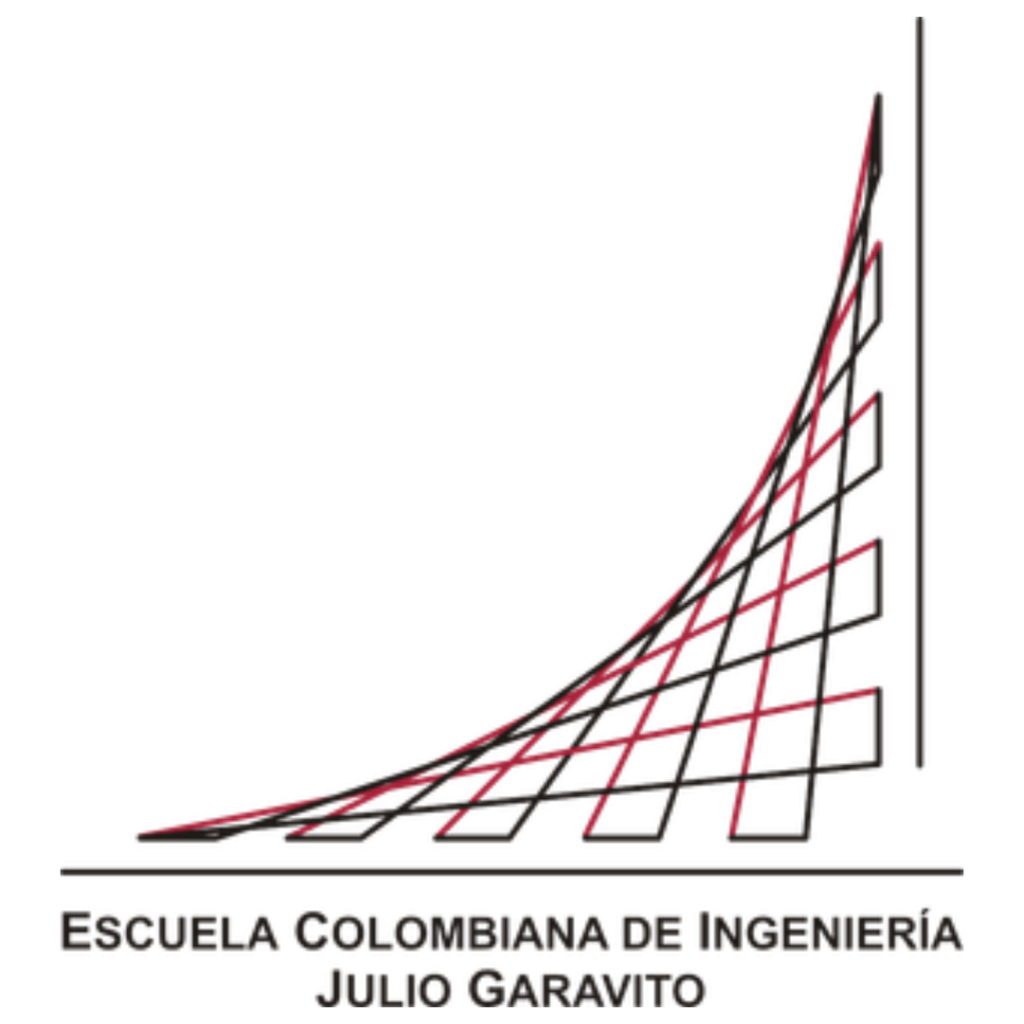
\includegraphics[width=2.5cm]{img/logo_eci_h.png} % AGREGAMOS EL LOGO UC
\vspace*{-2.2cm} % Esta linea va con la anterior


\begin{tabular}{l}
\hspace{2.5cm} ESCUELA COLOMBIANA DE INGENIERÍA JULIO GARAVITO\\
\hspace{2.5cm} DEPARTAMENTO DE INGENIERÍA DE SISTEMAS\\
\end{tabular}

\begin{center}
\vspace{3cm}
{\scshape\Huge \textbf{Nombre del proyecto} \par}
\rule{80mm}{0.1mm}
%\vspace{1cm}

{\itshape\LARGE Proyecto de curso PTIA \par}
\vfill
{\Large \textbf{Grupo XX} \par}
\vspace{0.5cm}
{\large \textbf{Integrantes:}\\\normalsize Nombre1, Nombre2, Nombre \par} 


\medskip
\textbf{Fecha de entrega:} <día> de <mes> de <año>
\vspace{3cm}
\end{center}
\end{titlepage}
\newpage
% Opcion 3: Sin portada - Se recomienda quitar indices

%%%%%%%%%%%%%%%%% PRELIMINARES %%%%%%%%%%%%%%%%

% El siguiente comando es usado para crear las cajas de firmas
\newcommand*\wildcard[2][6cm]{\vspace{2cm}\parbox{#1}{\hrulefill\par#2}} 

\section*{Declaración firmada}

\vspace{1cm}

“Declaro que he escrito este trabajo de investigación por mí mismo, y que no he utilizado otras fuentes o recursos que los indicados para su preparación. Declaro que he indicado claramente todas las citas directas e indirectas, y que este documento no se ha presentado en otro lugar para fines de examen o publicación"

\vspace{3cm}
\textbf{Nombre del estudiante \& Firma:}
\vspace{1cm}

\begingroup

    \begin{center}
        \wildcard{\centerline{<Nombre estudiante>} ~\\ \centerline{Fecha: <día> de <mes> de <año>}}
        \hspace{2cm} % "hspace{}"  para espacio horizontal entre misma fila
        \wildcard{\centerline{<Nombre estudiante>} ~\\ \centerline{Fecha: <día> de <mes> de <año>} }
    \end{center}

\endgroup


\pagebreak

%%%%%%%%%%%%%%%%% INDICES %%%%%%%%%%%%%%%%%
\setstretch{1}
\tableofcontents
\listoftables
\listoffigures
%\lstlistoflistings % Para hacer indice de codigo

%%%%%%%%%%%%%%%%% ESPACIADO %%%%%%%%%%%%%%%%%
\setstretch{1.15} 


%%%%%%%%%%%%%%%%% CONTENIDO %%%%%%%%%%%%%%%%%
\newpage
%\section{Comandos de \LaTeX}
Algunos de los principales comandos son:
\begin{table}[H]
    \centering
    \begin{tabular}{l l}
        \symbol{92}textit   & Permite escribir en \textit{itálica}. \\
        \symbol{92}textbf   & Permite poner en \textbf{negrilla} un texto. \\
        \symbol{92}sout     & Nos permite \sout{tachar} texto. \\
        \symbol{92}texttt   & Permite escribir texto con una \texttt{fuente monoespaciada}. \\
        \symbol{92}footnote & Permite agregar pies de página y una referencia a ella. \\
        \symbol{92}newpage  & Permite hacer un salto de página.\\
        \symbol{92}nameref{referencia} & Permite hacer referencias en el contenido\\
        \%     & Permite comentar todo texto que se encuentre a la derecha de este símbolo.
    \end{tabular}
\end{table}

%%%%%%%%%%%%%%%%%%%%%%%%%%%%%%%%%%%%%%%%%%%%%%%%%%%%%%%
\section{Organización}

\subsection{Referenciación}

Para referenciar en \LaTeX se usa el comando \symbol{92}cite . En el siguiente texto se puede apreciar unos ejemplos

\textcolor{RoyalBlue}{
Better predictive modeling depends on better understanding of the data and attributes selection. We have to choose between some data mining algorithm. We have chosen data mining as it is very much flexible in predictive modeling. Prediction when the game is in progress is a tough ask and it need finding the best attributes that influence the match outcome. Some research was done previously on predictive modeling in sports like Basketball, Baseball along with Test and One Day International cricket. \\ \\
In basketball, Bhandari et al.\cite{Bhandari1997} developed a knowledge discovery system and data mining framework for National Basketball Association (NBA). It was aimed to discover several interesting patterns in basketball games. This and related system have been used by several basketball teams over the past decades. Such solutions designed for offline usage and no in game effects were taken care of. There has been some recent works (20) about in-game decision making to find how much time remaining in the game without making any prior prediction model. \\ \\
There were several works done in cricket. Bailey and Clarke\cite{Bailey} and Sankaranarayanan et al.\cite{Sankaranarayanan} used machine learning approach to predict the result of a one day match depending on the previous data and in game data.}

\subsection{Secciones}
Pueden organizar el documento en distintas secciones y sub-secciones, lo que nos permite tener todo más ordenado, facilitando así la lectura. Actualmente, existen los siguientes niveles de organización:

\begin{table}[H]
    \centering
    \begin{tabular}{l l}
        \symbol{92}section\{\}       & \Large{\textbf{1.\hspace{.5cm} Secciones}} \\
        \symbol{92}subsection\{\}    & \large{\textbf{1.1.\hspace{.3cm} Subsecciones}} \\
        \symbol{92}subsubsection\{\} & \textbf{1.1.1.\hspace{.05cm} Subsubsecciones} \\
    \end{tabular}
\end{table}

\subsection{Listados}
Hay diferentes formas de listar elementos\footnote{Pueden usarse varias cosas, más info en el siguiente \href{https://es.overleaf.com/learn/latex/Lists}{link}}
\begin{multicols}{3}
    Uso de \texttt{itemize}
    \begin{itemize}
        \centering
        \item Elemento
        \item Elemento
        \item Elemento
    \end{itemize}
    
    \columnbreak % Para separar columna
    
    Uso de \texttt{enumerate}
    \begin{enumerate}
        \centering
        \item Elemento
        \item Elemento
        \item Elemento
    \end{enumerate}
    
    \columnbreak% Para separar columna x2
    
    Uso de elemento personalizado
    \begin{itemize}[$\blacksquare$] % o *, +, o, etc
        \centering
        \item Descripción
        \item Descripción
        \item Descripción
    \end{itemize}
\end{multicols}


%%%%%%%%%%%%%%%%%%%%%%%%%%%%%%%%%%%%%%%%%%%%%%%%%%%%%%%
\newpage
\section{Imágenes}
\subsection{Imagen centrada}
En esta plantilla hay 2 formas de incluir imágenes. La primera es la más compleja y manual que aparece en el código comentado.
%\begin{figure}[H] % IMPORTANTE en la mayoria de los casos, alternativas: [h],[t],[b],[p],
%    \centering
%    \begin{measuredfigure} % Lo usamos para aliniar el caption
%        \caption{Título de la imagen} % IMPORTANTE que este arriba
%        
\includegraphics[width=0.2\textwidth]{img/cuadradoejemplo.png} % Alternativa \includegraphics[height=3cm]{}
%        \label{img:referencia0}
%    \end{measuredfigure}
%\end{figure}

La segunda forma de incluir imágenes es la más sencilla, solo se tiene que usar el comando personalizado:
\begin{verbatim} 
\fig[label]{Titulo}{tamaño}{ruta_imagen}
Ejemplo:
\fig[referencia1]{Titulo de la imagen 1}{width = 0.2\textwidth}{img/cuadradoejemplo.png}
\end{verbatim}

\fig[referencia1]{Titulo de la imagen 1}{width = 0.2\textwidth}{img/cuadradoejemplo.png}

% Tambien se puede agregar sin caption ni label ni titulo:
% \fig{}{width = 0.2\textwidth}{img/cuadradoejemplo.png}

\subsection{Imágenes alineadas}
Si se desea incluir una imagen a la izquierda o derecha de un párrafo, se puede consultar nuevamente el codigo comentado o usar el siguiente comando (Poniendo \{r\} o \{l\} dependiendo del caso):
\begin{verbatim} 
\figposition[label]{Titulo}{tamaño}{ruta_imagen}{posicion_r/l}
Ejemplo:
\figposition[referencia2]{Imagen referencia }{height=3cm}{img/cuadradoejemplo.png}{r}
\end{verbatim}

\figposition[referencia2]{Imagen referencia }{height=3cm}{img/cuadradoejemplo.png}{r}

% FORMA MANUAL:
%\begin{wrapfigure}{r}{0.25\textwidth} % Margen del texto
%    \centering
%    \begin{measuredfigure}
%        \caption{Imagen referencia 2}
%        
\includegraphics[height=3cm]{img/cuadradoejemplo.png} %[scale=0.1]
%        \label{img:referencia2}
%    \end{measuredfigure}
%\end{wrapfigure}


\textcolor{silver}{
    Ahora generaremos algo de texto aleatorio...
    \lipsum[2]
}

\subsection{Imágenes que rompen márgenes}

Este es un caso muy particular, en el que se quiera incluir una imagen decorativa en algún estilo. En este caso de ejemplo, incluiremos una imagen en la base ([b]) al "south east", aunque también se puede incluir en "west" y personalizar de otras maneras.

\begin{figure}[b]
    \begin{tikzpicture}[remember picture, overlay]
    \node[anchor=south east, % west
        xshift=0mm,
        yshift=0mm,
        opacity=1]
        at (current page.south east)  % west
        {
\includegraphics[height=3cm]{img/cuadradoejemplo.png}};
        %(box) at (-2cm,0)(box){\includegraphics[scale=1]{img/circulos-amarillo3.png}};
    \end{tikzpicture}
    %\caption{Ilustración}
    %\label{fig:Ilustración}
\end{figure}

\newpage

%%%%%%%%%%%%%%%%%%%%%%%%%%%%%%%%%%%%%%%%%%%%%%%%%%%%%%%
\section{Tablas}

Hacer tablas en \LaTeX es muy engorroso, por lo que presentamos 3 alternativas. Sin embargo, es necesario aclarar que para que se respete el formato de las tablas, \textbf{se tiene que poner el catión SOBRE la tabla.}

\subsection{Generador online}
Hay muchas páginas para generar tablas automáticamente, una alternativa es \href{https://www.tablesgenerator.com}{tablesgenerator}, sin embargo, este método genera muchas líneas innecesarias y cuando se incorporan párrafos muy grandes hay que ajustar las palabras.

\subsection{Insertar una imagen como tabla}
Se puede incorporar una imagen (De Excel, por ejemplo) como si fuera una tabla. El único inconveniente es que no va a permitir seleccionar el texto en el pdf generado. Al igual que con las imágenes, hay un comando personalizado y un código manual comentado.\footnote{\textit{Si no se quiere incluir el texto opcional, pueden dejar vacío la última celda (\{\})}}
\begin{verbatim} 
\tableimage[label]{Titulo}{tamaño}{ruta_imagen}{Texto_referencia}
Ejemplo:
\tableimage[referencia3]{Tabla de referencia 1}{height=3cm}{img/tablaejemplo.png}{Texto}
\end{verbatim}



\tableimage[referencia3]{Titulo de la tabla de referencia}{height=3cm}{img/tablaejemplo.png}{Texto opcional con fuente/explicación.}

% Tabla manual:
%\begin{table}[H]
%    \centering
%    \begin{measuredfigure}
%        \caption{Tabla de referencia 1}
%        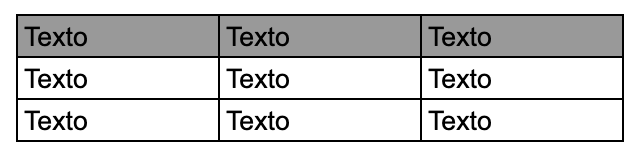
\includegraphics[height=3cm]{img/tablaejemplo.png} 
%        \label{img:referencia3}
%    \end{measuredfigure}
%    \\ \textit{\scriptsize{Texto opcional al el pie de Tabla.}}
%\end{table}


\subsection{Usar plantilas}
\begin{minipage}[H]{0.49\textwidth}
    \begin{table}[H]
        \centering
        \begin{measuredfigure}
            \caption{Tabla de referencia 2}
            \begin{tabular}{| l | c | r |} 
            \hline
                \textbf{Texto} & \textbf{Texto} & \textbf{Texto} \\ \hline
                Textoblabla    & Textoblabla   & Textoblabla \\ \hline
                Texto    & Texto   & Texto \\ \hline
            \end{tabular}
        \end{measuredfigure}
        \\ \textit{\scriptsize{Texto opcional al el pie de Tabla.}}
    \end{table}
\end{minipage}
\begin{minipage}[H]{0.49\textwidth}
    \begin{table}[H]
        \centering
        \begin{measuredfigure}
            \caption{Tabla de referencia 3}
            \begin{tabular}{l l l}
            \toprule
                \textbf{Texto} & \textbf{Texto} & \textbf{Texto} \\
                \midrule
                Textoblabla    & Textoblabla   & Textoblabla \\
                Texto    & Texto   & Texto \\
                \bottomrule
            \end{tabular}
        \end{measuredfigure}
        \\ \textit{\scriptsize{Texto opcional al el pie de Tabla.}}
    \end{table}
\end{minipage}

%%%%%%%%%%%%%%%%%%%%%%%%%%%%%%%%%%%%%%%%%%%%%%%%%%%%%%%
\newpage
\section{Código}
\subsection{pseudocódigo}
Para generar un pseudo código en blanco y negro se pueden basar en el siguiente estilo (Es importante la tabulación):

\texttt{PSEUDOCODIGO(A)} % Lo recomiendo defar fuera
\begin{lstlisting}[style=blancoynegro]
    i = 3
    while A <= i do
        print uwu
        i --
    end while
\end{lstlisting}

\subsection{Python}
Para escribir código como si fuera Python, se pueden basar en el siguiente estilo:
\begin{lstlisting}[language=Python, style=stylepython]
    def funcionpython(A):
        i = 3
        while True:
            print("UwU") # OwO
\end{lstlisting}

\subsection{json}
\begin{minted}[linenos,frame=single]{json} 
[
  {
    "palabra": "texto",
    "palabra": "texto",
    "id": 0
  }
]
\end{minted}

\subsection{Alternativa}
Sí usamos \symbol{92}begin\{verbatim\} podemos organizar con comodidad.
\begin{verbatim}
    1
    HOLA 4
    20 3
    FIN
\end{verbatim}

% Si se quiere poner \ se puede usar \symbol{92}

%%%%%%%%%%%%%%%%%%%%%%%%%%%%%%%%%%%%%%%%%%%%%%%%%%%%%%%
\newpage
\section{Cajas de texto}
Usando \texttt{tcolorbox} se pueden hacer diferentes cajas para incluir ejemplos, teoremas y demás. Acá adjunto algunos ejemplos de internet.

\begin{tcolorbox}
  Mi caja.
\end{tcolorbox}

\begin{tcolorbox}[colback=red!5!white,colframe=red!75!black]
  Mi caja x2.
\end{tcolorbox}

\begin{tcolorbox}[colback=blue!5!white,colframe=blue!75!black,title=Mi titulo]
  Mi caja con titulo
\end{tcolorbox}

\begin{tcolorbox}[colback=green!5!white,colframe=green!75!black]
  Parte superior
  \tcblower
  Parte inferior
\end{tcolorbox}

\begin{tcolorbox}[colback=yellow!5!white,colframe=yellow!50!black,colbacktitle=yellow!75!black,sidebyside,title=Mi titulo]
  Parte izquierda (agregada con "sidebyside")
  \tcblower
  Parte derecha
\end{tcolorbox}

\begin{tcolorbox}[colback=yellow!10!white,colframe=red!75!black,lowerbox=invisible,
  savelowerto=\jobname_ex.tex]
  Parte superior
  \tcblower
  Soy un texto invisible
\end{tcolorbox}

\begin{tcolorbox}[colback=yellow!10!white,colframe=red!75!black,title=Aparece el titulo invisible]
  \input{\jobname_ex.tex}
\end{tcolorbox}


%----------------------------------------------------------
\begin{tcolorbox}[enhanced,watermark graphics=img/cuadradoejemplo.png, watermark opacity=0.3,watermark zoom=0.9, colback=green!5!white,colframe=green!75!black, fonttitle=\bfseries, title=Titulo]
      Soy un texto creado solo para rellenar esta caja y mostrar que en el fondo hay una imagen como mascara y oculta con un degrade.
\end{tcolorbox}

%----------------------------------------------------------
\begin{tcolorbox}[colback=yellow!10!white,colframe=yellow!50!black,every box/.style={fonttitle=\bfseries},title=Caja1]
  \begin{tcolorbox}[enhanced,colback=red!10!white,colframe=red!50!black,colbacktitle=red!85!black,title=Caja2]
    \begin{tcolorbox}[beamer,colframe=blue!50!black,title=Caja3]
      Soy un texto de ejemplo!\par\medskip
      \newtcbox{\mybox}[1][]{nobeforeafter,tcbox raise base,colframe=green!50!black,colback=green!10!white,sharp corners,top=1pt,bottom=1pt,before upper=\strut,#1}
      \mybox[rounded corners=west]{Esta}
      \mybox{es}
      \mybox{una}
      \mybox[rounded corners=east]{caja!}
    \end{tcolorbox}
  \end{tcolorbox}
\end{tcolorbox}

\pagebreak % HABILITAR Y DESHABILITAR PARA TENER EJEMPLOS
\section{Introducción}

\begin{tcolorbox}[colback=yellow!10!white,colframe=red!75!black,title=Recomendaciones]
  Definición de los problemas
  \begin{itemize}
      \item ¿Cuáles serían tres problemas que les interesaría resolver?
      \item ¿Por qué como proyecto de PTIA?
  \end{itemize}
\end{tcolorbox}

\pagebreak
\section{Trabajos relacionados}

\begin{tcolorbox}[colback=yellow!10!white,colframe=red!75!black,title=Recomendaciones]
  Definir el estado del arte
  \begin{itemize}
      \item ¿Cuáles son dos trabajos relacionados a cada problema? (resultados y tecnología)
  \end{itemize}
\end{tcolorbox}

\pagebreak
\section{Descripción del problema}

\begin{tcolorbox}[colback=yellow!10!white,colframe=red!75!black,title=Recomendaciones]
  \begin{itemize}
      \item ¿Cuáles criterios van a usar para seleccionar el problema a resolver?
      \item ¿Cuál es el problema seleccionado?
  \end{itemize}
\end{tcolorbox}

\pagebreak
\section{Descripción del problema}

\begin{tcolorbox}[colback=yellow!10!white,colframe=red!75!black,title=Recomendaciones]
  \begin{itemize}
      \item ¿Cuál es el gran problema que se quiere resolver?
      \item ¿Por qué es importante resolverlo?
  \end{itemize}
\end{tcolorbox}

\pagebreak
\section{Alcance y Objetivos}

\begin{tcolorbox}[colback=yellow!10!white,colframe=red!75!black,title=Recomendaciones]
  \begin{itemize}
      \item ¿Cuál es el problema que efectivamente van a resolver?
      \item ¿Por qué consideran que es una simplificación adecuada?
      \item ¿Cuál sería el objetivo (cuantitativo y cualitativo)? Detallar objetivo general
  \end{itemize}
\end{tcolorbox}

\pagebreak
\section{Diseño metodológico}

\begin{tcolorbox}[colback=yellow!10!white,colframe=red!75!black,title=Recomendaciones]
Definir el paso a paso como se planear dar solución al problema
  \begin{itemize}
      \item ¿Cuál es la estrategia general seleccionada para la solución? Justificación
      \item ¿Dónde se concentra la inteligencia de la solución? (conocimiento+razonamiento) 
      \item ¿Qué herramienta seleccionaron para implementar la solución? Justificación
      \item ¿Cuál es la arquitectura de la solución? (Componentes y relaciones)
      \item ¿Cuál es el componente principal? (Descripción detallada)
  \end{itemize}
\end{tcolorbox}

\pagebreak
\section{Análisis de resultados}

\begin{tcolorbox}[colback=yellow!10!white,colframe=red!75!black,title=Recomendaciones]
Detallar los resultados
  \begin{itemize}
      \item ¿Cuáles son los dos mejores casos de prueba? (Secuencia de entradas y salidas esperadas y logradas)
      \item ¿Cuál es el caso de prueba más significativo? (Además de la secuencia de entradas y salidas, analicen el resultado)
  \end{itemize}
\end{tcolorbox}

\pagebreak
\section{Análisis de resultados}

\begin{tcolorbox}[colback=yellow!10!white,colframe=red!75!black,title=Recomendaciones]
Presentar una reflexión sobre los resultados y hallazgos de su trabajo; lecciones aprendidas
  \begin{itemize}
      \item ¿Cuáles son los dos aciertos y dos errores más relevantes? (Aprendizaje de cada uno de ellos)
      \item ¿Cuáles son las tres conclusiones más evidentes?
      \item ¿Cuál es una buena idea de trabajo futuro?
  \end{itemize}
  
  \textit{Las conclusiones son una oportunidad para resumir los resultados y hallazgos de una investigación o un proyecto, y para hacer énfasis en la idea o punto principal del escrito al final de su argumento}
\end{tcolorbox}

\pagebreak


%%%%%%%%%%%%%%%%% BIBLIOGRAFIA %%%%%%%%%%%%%%%%%
\newpage
\printbibliography

%%%%%%%%%%%%%%%%%%% ANEXOS %%%%%%%%%%%%%%%%%%%%%

\newpage
%% ************************************************ %
%              ANEXO INSTALACIÓN LATEX             %
% ************************************************ %

\section*{How to install \LaTeX} 

\subsection*{Windows OS}

\subsubsection*{TeXLive package - full version}
\begin{enumerate}
\item	Download the TeXLive ISO (2.2GB) from\\
\href{https://www.tug.org/texlive/}{https://www.tug.org/texlive/}
\item	Download WinCDEmu (if you don't have a virtual drive) from \\
\href{http://wincdemu.sysprogs.org/download/}
{http://wincdemu.sysprogs.org/download/}
\item	To install Windows CD Emulator follow the instructions at\\
\href{http://wincdemu.sysprogs.org/tutorials/install/}
{http://wincdemu.sysprogs.org/tutorials/install/}
\item	Right click the iso and mount it using the WinCDEmu as shown in \\
\href{http://wincdemu.sysprogs.org/tutorials/mount/}{
http://wincdemu.sysprogs.org/tutorials/mount/}
\item	Open your virtual drive and run setup.pl
\end{enumerate}

or

\subsubsection*{Basic MikTeX - \TeX~ distribution}
\begin{enumerate}
\item	Download Basic-MiK\TeX (32bit or 64bit) from\\
\href{http://miktex.org/download}{http://miktex.org/download}
\item	Run the installer 
\item	To add a new package go to Start >> All Programs >> MikTex >> Maintenance (Admin) and choose Package Manager
\item	Select or search for packages to install
\end{enumerate}

\subsubsection*{TexStudio - \TeX~ editor}
\begin{enumerate}
\item	Download TexStudio from\\
\href{http://texstudio.sourceforge.net/\#downloads}
{http://texstudio.sourceforge.net/\#downloads} 
\item	Run the installer
\end{enumerate}

\subsection*{Mac OS X}

\subsubsection*{MacTeX - \TeX~ distribution}
\begin{enumerate}
\item	Download the file from\\
\href{https://www.tug.org/mactex/}{https://www.tug.org/mactex/}
\item	Extract and double click to run the installer. It does the entire configuration, sit back and relax.
\end{enumerate}

\subsubsection*{TexStudio - \TeX~ editor}
\begin{enumerate}
\item	Download TexStudio from\\
\href{http://texstudio.sourceforge.net/\#downloads}
{http://texstudio.sourceforge.net/\#downloads} 
\item	Extract and Start
\end{enumerate}


\subsection*{Unix/Linux}

\subsubsection*{TeXLive - \TeX~ distribution}

\paragraph{Getting the distribution:}
\begin{enumerate}
\item	TexLive can be downloaded from\\
\href{http://www.tug.org/texlive/acquire-netinstall.html}
{http://www.tug.org/texlive/acquire-netinstall.html}.
\item	TexLive is provided by most operating system you can use (rpm,apt-get or yum) to get TexLive distributions
\end{enumerate}

\paragraph{Installation}
\begin{enumerate}
\item	Mount the ISO file in the mnt directory
\begin{verbatim}
mount -t iso9660 -o ro,loop,noauto /your/texlive####.iso /mnt
\end{verbatim}

\item	Install wget on your OS (use rpm, apt-get or yum install)
\item	Run the installer script install-tl.
\begin{verbatim}
	cd /your/download/directory
	./install-tl
\end{verbatim}
\item	Enter command `i' for installation

\item	Post-Installation configuration:\\
\href{http://www.tug.org/texlive/doc/texlive-en/texlive-en.html\#x1-320003.4.1}
{http://www.tug.org/texlive/doc/texlive-en/texlive-en.html\#x1-320003.4.1} 
\item	Set the path for the directory of TexLive binaries in your .bashrc file
\end{enumerate}

\paragraph{For 32bit OS} ~\

For Bourne-compatible shells such as bash, and using Intel x86 GNU/Linux and a default directory setup as an example, the file to edit might be

\begin{verbatim}
edit $~/.bashrc file and add following lines
PATH=/usr/local/texlive/2011/bin/i386-linux:$PATH; 
export PATH 
MANPATH=/usr/local/texlive/2011/texmf/doc/man:$MANPATH;
export MANPATH 
INFOPATH=/usr/local/texlive/2011/texmf/doc/info:$INFOPATH;
export INFOPATH
\end{verbatim}

\paragraph{For 64bit OS}
\begin{verbatim}
edit $~/.bashrc file and add following lines
PATH=/usr/local/texlive/2011/bin/x86_64-linux:$PATH;
export PATH 
MANPATH=/usr/local/texlive/2011/texmf/doc/man:$MANPATH;
export MANPATH 
INFOPATH=/usr/local/texlive/2011/texmf/doc/info:$INFOPATH;
export INFOPATH

\end{verbatim}



%\subsection{Installing directly using Linux packages} 
\paragraph{Fedora/RedHat/CentOS:}
\begin{verbatim} 
sudo yum install texlive 
sudo yum install psutils 
\end{verbatim}


\paragraph{SUSE:}
\begin{verbatim}
sudo zypper install texlive
\end{verbatim}


\paragraph{Debian/Ubuntu:}
\begin{verbatim} 
sudo apt-get install texlive texlive-latex-extra 
sudo apt-get install psutils
\end{verbatim} % HABILITAR Y DESHABILITAR PARA TENER EJEMPLOS

\end{document}